\documentclass[aspectratio=169, handout]{beamer}

% PACKAGES -----------------------------------------------------------------------------------------

\usepackage{array}
\usepackage[export]{adjustbox}
\usepackage{caption}
\usepackage{listings}
\usepackage{ragged2e}
\usepackage{pgfplots}
\usepackage{setspace}
\usepackage[dvipsnames]{xcolor}
\usepackage{multirow}
\usepackage{hyperref}

\usetikzlibrary{patterns}

% THEMING ------------------------------------------------------------------------------------------

% Beamer slide structure
\usetheme{Madrid}
\setbeamertemplate{navigation symbols}{}
\setbeamertemplate{caption}[numbered]
\setbeamertemplate{caption label separator}[period]

% Beamer colors
\usecolortheme{beaver}
\setbeamercolor{item}{fg=darkred}
\setbeamercolor{section in head/foot}{bg = white}

% Beamer header
\addtobeamertemplate{frametitle}{\vspace{-0.2ex}}{\vspace{0.5ex}}
\setbeamercolor{frametitle}{fg=darkred,bg=}

% Beamer footer
\setbeamercolor{footer}{bg = white, fg = black}
\setbeamertemplate{footline}{
    \hbox{%
        \begin{beamercolorbox}[wd=.333333\paperwidth,ht=2.25ex,dp=1ex,left]{footer}
            \hspace{2ex}\insertshortauthor
        \end{beamercolorbox}%
        \begin{beamercolorbox}[wd=.333333\paperwidth,ht=2.25ex,dp=1ex,center]{footer}
            \insertshorttitle
        \end{beamercolorbox}%
        \begin{beamercolorbox}[wd=.333333\paperwidth,ht=2.25ex,dp=1ex,right]{footer}
            \insertframenumber\hspace{2ex}
        \end{beamercolorbox}
    }
}

% Code theming
\lstdefinestyle{codestyle}{
    language       = sql,
    keywordstyle   = \color{darkred},
    basicstyle     = \ttfamily\footnotesize,
    deletekeywords = {CLUSTER},
}

\lstset{style = codestyle}

% Other
\def\arraystretch{1.5}
\DeclareCaptionFont{darkred}{\color{darkred}}
\captionsetup{font=scriptsize,labelfont={darkred,scriptsize}}

% DOCUMENT INFORMATION -----------------------------------------------------------------------------

\title
    [High Performance Data Analysis 25/26]
    {\large Optimizing LLM Inference on Fujitsu A64FX CPUs}
\subtitle{\color{black} \small High Performance Data Analysis 25/26}

\author[Group 12]{
    \begin{tabular}{lc}
        Humberto Gomes & \color{gray} pg59806 \\
        José Lopes     & \color{gray} pg59807 \\
        José Soares    & \color{gray} pg60277
    \end{tabular}
}

\institute{
    Department of Informatics -- School of Engineering -- University of Minho \\
    \vspace{0.5\baselineskip}
    
\includegraphics[height=1cm]{res/SchoolOfEngineeringCropped.pdf}
}
\date{\scriptsize May 18\textsuperscript{th} 2026}

\newif\ifplacelogo
\logo{
    \ifplacelogo
        \begin{tikzpicture}[overlay, remember picture]
        \node[anchor=north east, inner sep = 0] at (current page.north east) {
            \LARGE
            
\includegraphics[height=1.1\baselineskip]{res/SchoolOfEngineeringCropped.pdf}
        };
        \end{tikzpicture}
    \fi
}

% DOCUMENT CONTENTS --------------------------------------------------------------------------------

\begin{document}

\placelogofalse
\frame[plain]{\titlepage}
\placelogotrue

\setcounter{framenumber}{0}
\justifying

\section{Introduction}

\begin{frame}{Introduction}
    \begin{itemize}
        \item AI workloads are increasingly predominant in HPC (11\% of EuroHPC hours);
        \item In Deucalion:
    \end{itemize}

    \vspace{1em}

    \begin{minipage}{0.48\textwidth}
        \centering
        \textbf{GPU partition} \\
        Insufficient to meet demand \\
        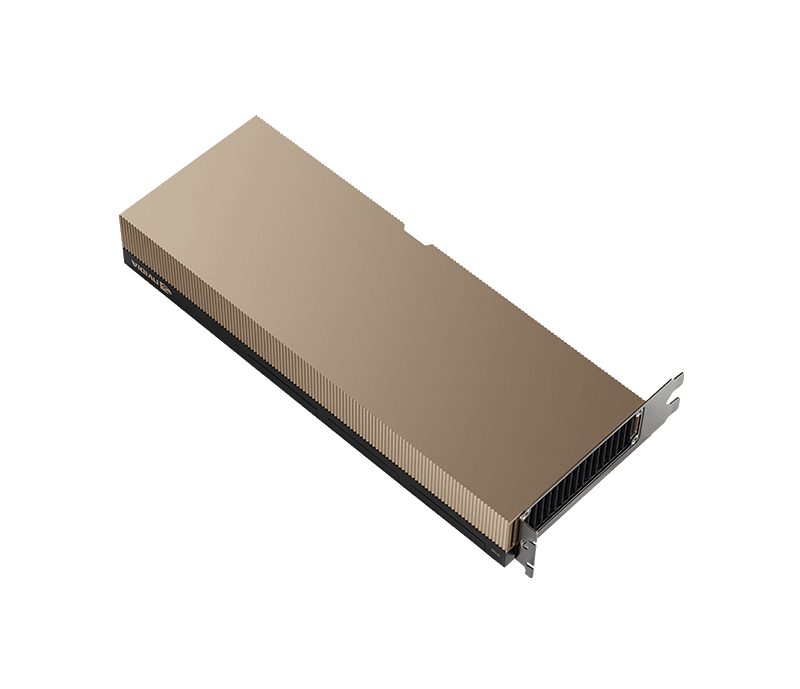
\includegraphics[height = 0.5\textwidth]{res/H100.png}
    \end{minipage}
    \begin{minipage}{0.48\textwidth}
        \centering
        \textbf{ARM partition (A64FX)} \\
        Requires optimization to be viable \\
        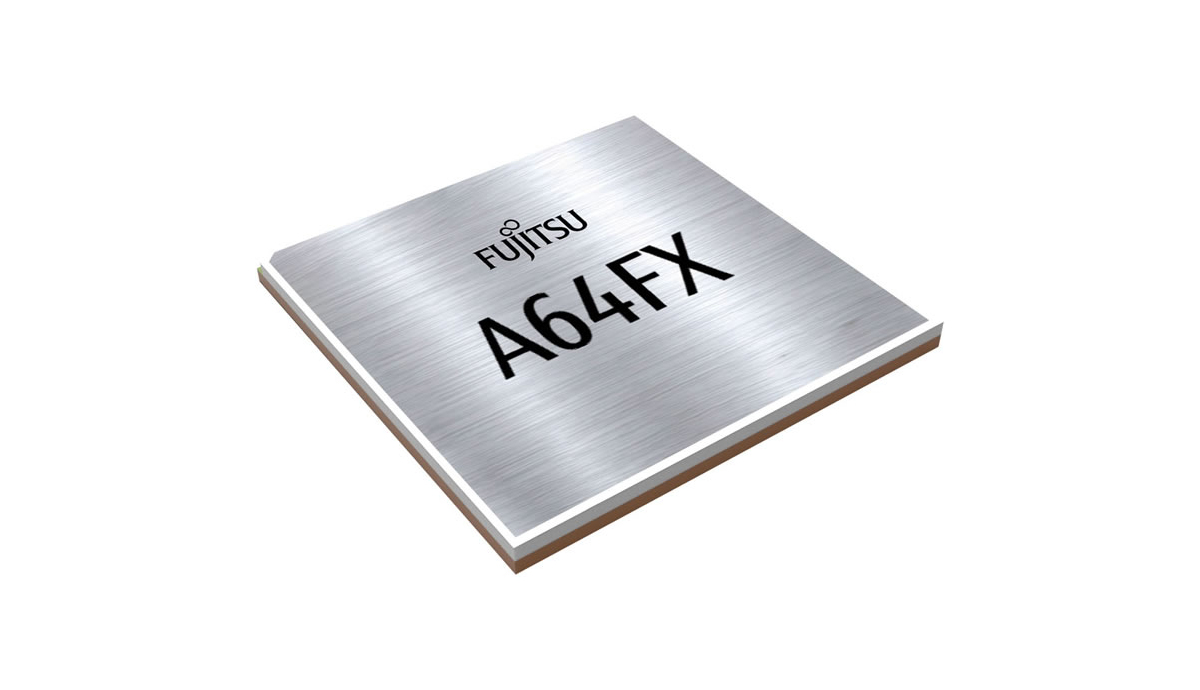
\includegraphics[height = 0.5\textwidth]{res/A64FX.jpg}
    \end{minipage}
\end{frame}

\section{Methodology}

\begin{frame}{Methodology}
    \begin{table}[H]
        \centering
        \begin{tabular}{|l|c|}
            \hline
            \textbf{Model}       &
            \textbf{Quantization} \\ \hline

            \texttt{SmolLM-2-135M-Instruct}                      &
            \texttt{Q3\_K\_M}, \texttt{Q4\_K\_M}, \texttt{Q8\_0} \\ \hline

            \texttt{Gemma-3-4B-Instruct}                         &
            \texttt{Q3\_K\_M}, \texttt{Q4\_K\_M}, \texttt{Q8\_0} \\ \hline

            \texttt{Meta-Llama-3.1-8B-Instruct}                  &
            \texttt{Q3\_K\_M}, \texttt{Q4\_K\_M}, \texttt{Q8\_0} \\ \hline
        \end{tabular}

        \caption{LLMs selected for benchmarking.}
    \end{table}

    \begin{itemize}
        \item Inference engine: \texttt{llama.cpp} (\texttt{llama-server});
    \end{itemize}
\end{frame}

\section{Optimizations}

\begin{frame}{Compiler Configuration}
    \begin{minipage}{0.55\textwidth}
        \vspace{4ex}
        \begin{table}[H]
            \centering
            \begin{tabular}{|l|r|r|}
                \hline
                \textbf{Configuration} & \textbf{TTFT} & \textbf{TPOT} \\ \hline
                Clang + BLIS           &         1.057 &         1.004 \\ \hline
                Clang                  &         1.099 &         1.019 \\ \hline
                GCC + BLIS             &         1.104 &         1.371 \\ \hline
                GCC                    &         1.555 &         1.691 \\ \hline
            \end{tabular}
            \caption{
                \onehalfspacing
                Geometric mean of TTFT and TPOT, normalized to the best compiler per benchmark.
            }
            \label{compiler-geomean}
        \end{table}
    \end{minipage}
    \begin{minipage}{0.4\textwidth}
        \vspace{-2ex}
        \centering
        \large
        \textbf{Clang + BLIS}\\
        \vspace{1ex}
        \normalsize \color{black} reduction in TPOT up to \\
        \vspace{1ex}
        \color{ForestGreen}\Huge + $68.5\%$\\
    \end{minipage}
\end{frame}

\begin{frame}{Model Quantization}
    \begin{minipage}{0.48\textwidth}
        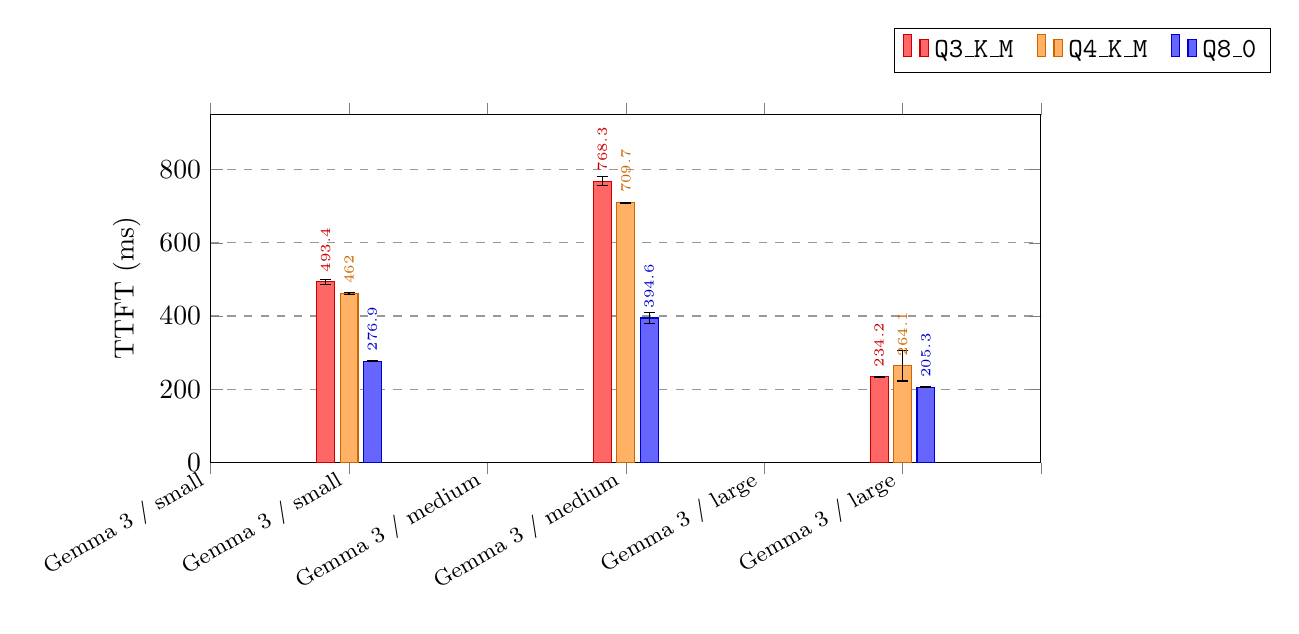
\begin{tikzpicture}
            \begin{axis}[
                % Plot type
                ybar,
                % Plot dimensions
                width            = \textwidth,
                height           = 6cm,
                enlarge x limits = 0.25,
                bar width        = 1.5ex,
                % Labels
                ylabel            = {TTFT (ms)},
                symbolic x coords = {
                    {Gemma 3 / small},
                    {Gemma 3 / medium},
                    {Gemma 3 / large},
                },
                x tick label style = {rotate = 30, anchor = east, font = \footnotesize},
                % Axes
                ymin = 0,
                ymax = 950,
                % Labels
                nodes near coords,
                nodes near coords style={
                    font   = \tiny,
                    rotate = 90,
                    anchor = west,
                    /pgf/number format/fixed,
                    /pgf/number format/precision = 1
                },
                % Grid
                ymajorgrids = true,
                grid style  = {dashed, gray!80},
                % Legend
                legend style = {
                    at             = {(1.05, 1.25)},   % desloca para o meio dos dois plots
                    anchor         = north,
                    legend columns = 3,
                    /tikz/every even column/.append style = {column sep = 1.5ex}
                }
            ]

                % Q3_K_M
                \addplot+[
                    % Bar and label color
                    fill                                = red!60,
                    draw                                = red!80!black,
                    every node near coord/.append style = {color = red!80!black},
                    % Error bars
                    error bars/.cd,
                    y dir = both,
                    y explicit,
                    error bar style = {black, line width = 0.5pt}
                ] coordinates {
                    ({Gemma 3 / small},     493.38) +- (0,   6.46)
                    ({Gemma 3 / medium},    768.28) +- (0,  12.75)
                    ({Gemma 3 / large},     234.16) +- (0,   0.92)
                };

                % Q4_K_M
                \addplot+[
                    % Bar and label color
                    fill                                = orange!60,
                    draw                                = orange!80!black,
                    every node near coord/.append style = {color = orange!80!black},
                    % Error bars
                    error bars/.cd,
                    y dir = both,
                    y explicit,
                    error bar style = {black, line width = 0.5pt}
                ] coordinates {
                    ({Gemma 3 / small},     462.04) +- (0,   3.19)
                    ({Gemma 3 / medium},    709.74) +- (0,   1.52)
                    ({Gemma 3 / large},     264.12) +- (0,  41.54)
                };

                % Q8_0
                \addplot+[
                    % Bar and label color
                    fill                                = blue!60,
                    draw                                = blue!80!black,
                    every node near coord/.append style = {color = blue!80!black},
                    % Error bars
                    error bars/.cd,
                    y dir = both,
                    y explicit,
                    error bar style = {black, line width = 0.5pt}
                ] coordinates {
                    ({Gemma 3 / small},     276.87) +- (0,   1.75)
                    ({Gemma 3 / medium},    394.57) +- (0,  14.23)
                    ({Gemma 3 / large},     205.31) +- (0,   1.23)
                };

                \legend{\texttt{Q3\_K\_M}, \texttt{Q4\_K\_M}, \texttt{Q8\_0}}
            \end{axis}
        \end{tikzpicture}
    \end{minipage}
    \begin{minipage}{0.48\textwidth}
        \vspace{5ex}
        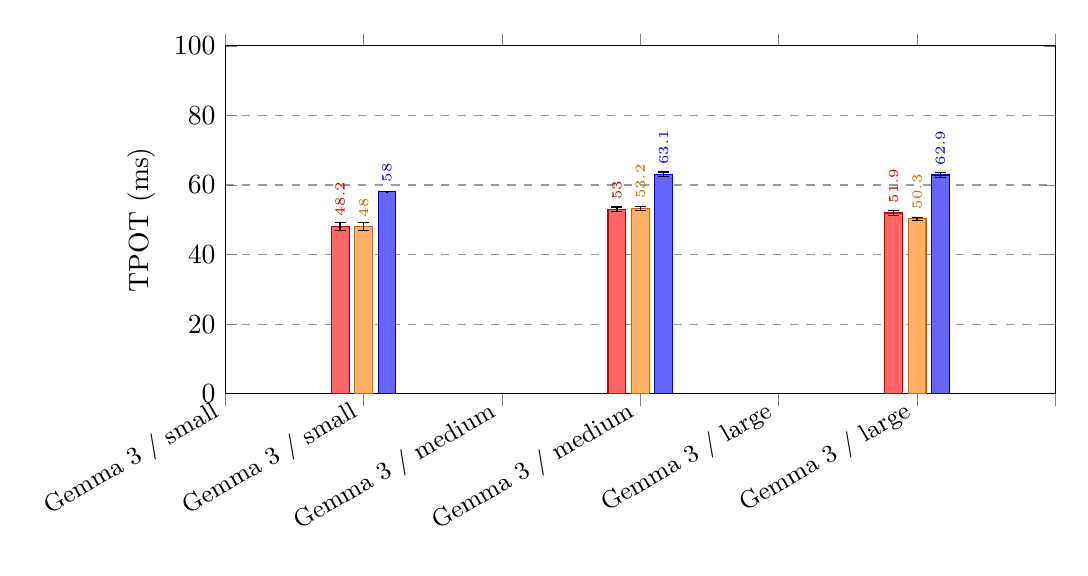
\begin{tikzpicture}
            \begin{axis}[
                % Plot type
                ybar,
                % Plot dimensions
                width            = \textwidth,
                height           = 6cm,
                enlarge x limits = 0.25,
                bar width        = 1.5ex,
                % Labels
                ylabel            = {TPOT (ms)},
                symbolic x coords = {
                    {Gemma 3 / small},
                    {Gemma 3 / medium},
                    {Gemma 3 / large},
                },
                x tick label style = {rotate = 30, anchor = east, font = \small},
                % Axes
                ymin = 0,
                ymax = 100,
                % Labels
                nodes near coords,
                nodes near coords style={
                    font   = \tiny,
                    rotate = 90,
                    anchor = west,
                    /pgf/number format/fixed,
                    /pgf/number format/precision = 1
                },
                % Grid
                ymajorgrids = true,
                grid style  = {dashed, gray!80}
            ]

                % Q3_K_M
                \addplot+[
                    % Bar and label color
                    fill                                = red!60,
                    draw                                = red!80!black,
                    every node near coord/.append style = {color = red!80!black},
                    % Error bars
                    error bars/.cd,
                    y dir = both,
                    y explicit,
                    error bar style = {black, line width = 0.5pt},
                ] coordinates {
                    ({Gemma 3 / small},      48.18) +- (0,  1.16)
                    ({Gemma 3 / medium},     52.97) +- (0,  0.71)
                    ({Gemma 3 / large},      51.94) +- (0,  0.65)
                };

                % Q4_K_M
                \addplot+[
                    % Bar and label color
                    fill                                = orange!60,
                    draw                                = orange!80!black,
                    every node near coord/.append style = {color = orange!80!black},
                    % Error bars
                    error bars/.cd,
                    y dir = both,
                    y explicit,
                    error bar style = {black, line width = 0.5pt},
                ] coordinates {
                    ({Gemma 3 / small},      47.97) +- (0, 1.12)
                    ({Gemma 3 / medium},     53.19) +- (0, 0.62)
                    ({Gemma 3 / large},      50.25) +- (0, 0.48)
                };

                % Q8_0
                \addplot+[
                    % Bar and label color
                    fill                                = blue!60,
                    draw                                = blue!80!black,
                    every node near coord/.append style = {color = blue!80!black},
                    % Error bars
                    error bars/.cd,
                    y dir = both,
                    y explicit,
                    error bar style = {black, line width=0.5pt},
                ] coordinates {
                    ({Gemma 3 / small},      58.04) +- (0, 0.02)
                    ({Gemma 3 / medium},     63.07) +- (0, 0.67)
                    ({Gemma 3 / large},      62.86) +- (0, 0.74)
                };
            \end{axis}
        \end{tikzpicture}
    \end{minipage}
\end{frame}

\begin{frame}{Threading and NUMA}
    \begin{table}[h]
        \centering
        \begin{tabular}{|c|c|r|r|}
            \hline
            \textbf{\emph{Threads}} & \textbf{NUMA}       & \textbf{TTFT} & \textbf{TPOT} \\ \hline
                                48 & \texttt{distribute} &        1.0424 &        1.0063 \\ \hline
                                44 & \texttt{distribute} &        1.0309 &        1.0293 \\ \hline
                                48 & Not defined         &        1.1764 &        1.0502 \\ \hline
                                36 & \texttt{distribute} &        1.1335 &        1.1158 \\ \hline
                                24 & \texttt{distribute} &        1.4689 &        1.4236 \\ \hline
                                12 & \texttt{distribute} &        2.4469 &        2.3407 \\ \hline
        \end{tabular}
        \caption{
            Geometric mean of TTFT and TPOT, normalized to the best threading configuration per
            benchmark.
        }
    \end{table}
\end{frame}

\begin{frame}{Performance Model}
    \centering
    $$
        \text{TPOT} \;\geq\; k \frac{M_{\text{RAM}}}{\text{BW}_{\text{mem}}}
    $$


    \vspace{4ex}

    \begin{table}[H]
        \centering
        \begin{tabular}{|l|r|r|r|r|r|}
            \hline
            \multirow{2}{*}{\textbf{Model}}          &
            \multirow{2}{*}{\textbf{Obs. (ms)}}      &
            \multicolumn{2}{c|}{\textbf{$k = 1$}}    &
            \multicolumn{2}{c|}{\textbf{$k = 9.27$}} \\ \cline{3-6}

                                &
                                &
            \textbf{Pred. (ms)} &
            \textbf{Error}      &
            \textbf{Pred. (ms)} &
            \textbf{Error}      \\ \hline

            \texttt{Llama 3.1} & 75.9 & 5.88 & 92.3\% & 50.35 & 33.7\% \\ \hline
            \texttt{Gemma 3}   & 52.5 & 3.19 & 93.9\% & 25.42 & 51.6\% \\ \hline
            \texttt{SmolLM 2}  &  9.3 & 0.59 & 93.7\% &  1.34 & 85.6\% \\ \hline
        \end{tabular}
        \caption{Predictions for \texttt{Q4\_K\_M} quantization.}
    \end{table}
\end{frame}

\section{Conclusions}

\begin{frame}{Conclusions}
    \begin{itemize}
        \item Largest gains came from systems-level tuning:
        \begin{itemize}
            \item \makebox[3cm]{Clang + BLIS\hfill}             $\rightarrow$ TPOT 68.5\% $\uparrow$;
            \item \makebox[3cm]{NUMA \texttt{distribute}\hfill} $\rightarrow$ TPOT 4.4\% $\uparrow$.
        \end{itemize}
        \item The analytical model underestimated TPOT by $7\times$--$19\times$;
        \item Many knobs left to tune and many improvements to \texttt{llama.cpp}.
    \end{itemize}

    \begin{center}
        \includegraphics[width = 0.3\textwidth]{res/neuralNetwork.png}
    \end{center}
\end{frame}

\placelogofalse
\frame[plain]{\titlepage}
\placelogotrue

\end{document}
